\section{Kapacitet} \label{kap}
% Skriv ift kapacitet (ift sengepladser, persona - hvilken betydning har hhv. 95 \% kapacitet mod 105 \%)
Kapacitetudnyttelse betegner forholdet mellem aktivitet og kapacitet. Aktivitet omhandler patient og kontakt, herunder består kontakt af forundersøgelse, behandling og kontrol. Kapacitet omfatter antallet af personale, udstyr og rum, hvor personalet består af læger, sygeplejersker og sekretærer. Udstyret beskriver antallet af maskiner på en afdeling og antallet af rum beskriver opbevarelsen af udstyret. Den samlede kapacitetsudnyttelse er defineret ud fra, at der produceres mest muligt for de investerede ressourcer.\cite{Company2013} 

\begin{figure}[H]
	\flushleft 
	\centering
	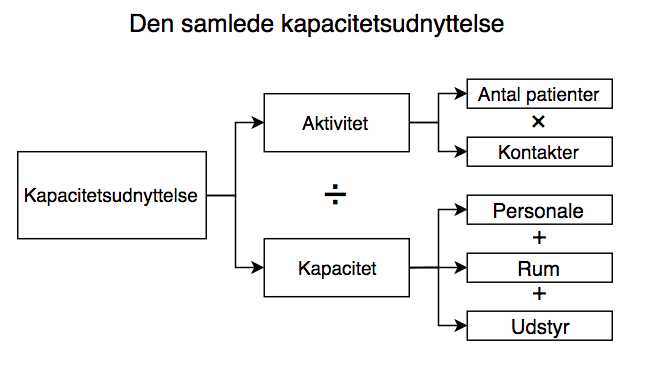
\includegraphics[scale=.7]{figures/Kapacitetsudnyttelse.png}
	\flushleft
	\caption{\textit{Den samlede kapacitetsudnyttelse som er definineret ved forholdet mellem aktivitet og kapacitet. Aktivitet omfatter antallet af patienter samt kontakter og kapacitet omfatter personale, rum og udstyr.}\cite{Company2013}}
	\label{kapacitet}
\end{figure}

\noindent
Ud fra \figref{kapacitet} fremgår det, at kapacitetsudnyttelse er forholdet mellem aktivitet og kapacitet. Dertil ses aktivitet som antal patienter multipliceret med kontakter. Kapaciteten udgør personale, rum og udstyr lagt sammen. Antallet af patienter, der repræsenterer en del af aktivitet beskriver ligeledes belægning på hospitalets afdelinger.\cite{Company2013} 

Belægning er defineret ud fra antallet af patienter, der er normeret til på en afdeling\cite{Heidmann2014}. Når en $100~\%$ belægning opnås, svarer dette til, at de disponible sengepladser på en afdeling er taget i brug. Ved en belægning på over $100~\%$ betyder det, at der er flere patienter end afdelingen er normeret til, hvilket vil sige, at afdelingen yder mere end der er kapacitet til. Ud fra \figref{kapacitet} vil dette betyde, at der ikke er ligevægt mellem aktivitet og kapacitet, hvilket i dette tilfælde vil forårsage kapacitetsmangel på afdelingen. Det kan derfor være nødvendigt, at personalet skal varetage flere patienter samt arbejdsopgaver, det kan ligeledes være nødvendigt at tilkalde ekstra personale for at opnå en balance i kapacitetsudnyttelsen.
Hvis der derimod er en belægning på under $100~\%$ er der omvendt færre patienter end afdelingen er normeret til. Dette betyder, at der er flere sengepladser end patienter, hvilket ligeledes fører til en ubalance i kapacitetsudnyttelsen. I denne situation er der mere personale end nødvendigt til at varetage de enkelte patienter, hvilket betyder, at der ikke er fuld udnyttelse af personalets arbejdskraft.\cite{Pauly1986} 

Det anses herved vigtigt, at der er balance mellem aktivitet og kapacitet, således de investerede ressourcer udnyttes optimalt. Det ønskes derfor at opnå en kapacitetsudnyttelse på 100\%. Ud fra dette vil der fremover undersøges betydningen af kapacitetsudnyttelse på ortopædkirurgisk afdeling på Aalborg Universitetshospital. 

\subsection{Ortopædkirurgisk afdeling}
Kapacitetsudnyttelse afhænger af det budget som hver afdeling har til rådighed. Dette budget udregner Sundhedsstyrrelsen ud fra diagnoserelaterede grupper (DRG). DRG anvendes til at analysere omkostninger og aktivitet på et hospital.\cite{DRG2016} Ortopædkirurgisk afdeling har et budget på $700.872.744$ kr, som svarer til 17,2 \% af det samlede budget for alle afdelinger på Aalborg Universitetshospital. Det samlede DRG for afdelingerne på Aalborg Universitetshospital er illusteret af \figref{DRG_budget}.\cite{Rasmussen2016}
Størstedelen af budgettet anvendes til personale- og patientudgifter, som svarer til hhv. 60 \% og 32 \%. Det resterende budget anvendes til bygninger, it, apparatur, inventar samt drift og service\cite{Noegletal2016}. 


\begin{figure}[H]
	\flushleft 
	\centering
	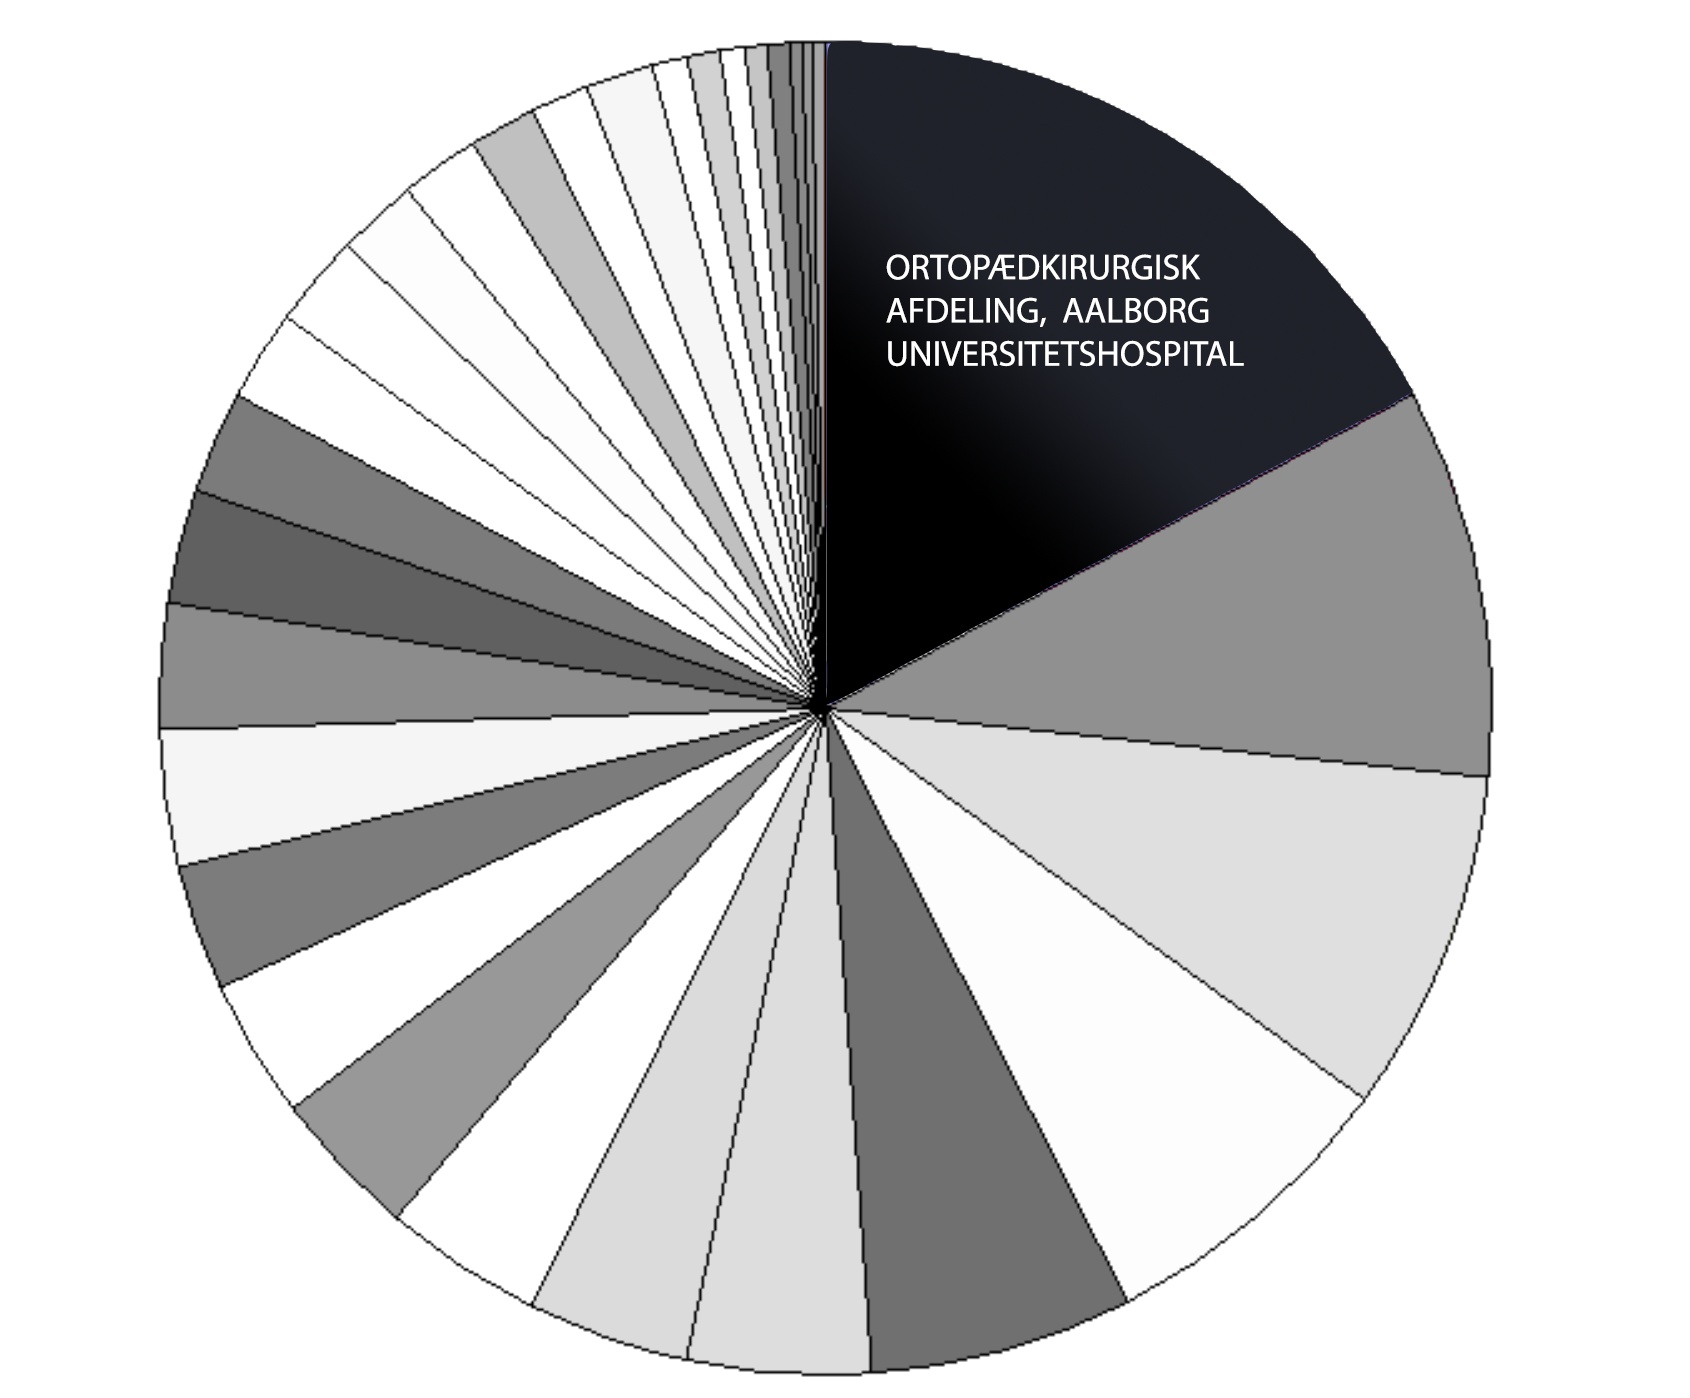
\includegraphics[scale=0.40]{figures/Ortopaeddiagram.png}
	\flushleft
	\caption{\textit{Fordeling af DRG for samtlige afdelinger på Aalborg Universitetshospital. Det fremgår, at ortopædkirurigisk afdeling har en større andel end de resterende afdelinger.}\cite{Rasmussen2016}}
	\label{DRG_budget}
\end{figure}


\subsubsection{Personalearbejde} 
% Hvordan opleves belægning generelt på OA på Aalborg UH? Hvordan varetages opgaver af personalet? Hvordan er vagtskifte? Hvor langt tid arbejdes der gennemsnitlig om dagen?
%Som beskrevet i \autoref{sec:kap} er personalet en del af kapacitet. Personalet ses som en væsentlig faktor for at udnytte kapaciteten effektivt. 
På ortopædkirurgisk afdeling på Aalborg Universitetshospital arbejder personalet i gennemsnit 37 timer om ugen\cite{Danske2015}. Vagterne kan variere fra XX til XX timer, hvoraf det både kan være nat- og dagvagter. Der er indlagt betalte pauser, hvilket betyder, at personalet skal være til rådighed under pausen. Pauserne er opdelt i XX om dagen. Afdelingen er delt op i XX vagthold og har vagtskifte hver XX time. Personalet varetager XX patienter om dagen. \fxnote{Vi mangler informationer for at kunne skrive dette færdigt.}

\subsubsection{Patientindlæggelse}
% Hvordan foregår indlæggelsen på OA på AUH? Hvornår indlæggelses patienterne (elektive patienter) og hvornår på dagen udskrives patienter (både elektive og akutte patienter) Hvor mange patienter hhv. akutte vs. elektive patienter? Hvad er deres buffer i forhold til elektive patienter, således der er plads til de akutte indlæggelser? indkaldes elektive patienter, hvis der er mindre akutte i en periode end der er estimeret til? Øges den normerede kapacitet under overbelægning ved at indkalde vikarbureau? (Altså tager man samme mængde elektive patienter ind.) 


Som beskrevet i afsnit \ref{kap} ønskes en 100\% kapacitetsudnyttelse, dertil ønskes ligeledes en belægning på 100\%. 
For at opfylde dette skal der være ligevægt mellem antallet af sengepladser og patientindlæggelser. På ortopædkirurgisk afdeling har de XX sengepladser til rådighed, som er fordelt på XX afsnit.

Ortopædkirurgisk afdeling modtager både elektive samt akutte patienter. Elektive patienter omfatter både indlagte og ambulante patienter. Ved pludselig forværret tilstand kan elektive patienter skifte status fra elektiv til akut. Akutte patienter defineres som personer, der er henvist til hospitalet efter en akut opstået tilstand. Sammenlignes der med de resterende afdelinger på Aalborg Universitetshospital, har ortopædkirurgisk afdeling flest elektive indlæggelser.\cite{RegionNord2016} Elektive patienter indlægges i tidsrummet XX-XX og udskrives i tidsrummet XX-XX. Udskrivelsen af akutte patienter foregår i samme tidsrum. På afdelingen planlægges elektive patienter med forbehold for, at der er uforudsigelige indlæggelser af akutte patienter pr. XX. Herunder planlægges XX elektive patienter, således at der er plads til XX akutte patienter.\fxnote{Vi mangler informationer for at kunne skrive dette færdigt + tilføjelse af Sebastians grafer (elektive/akuttte) + (indlæggelse/udskrivelse)}